\documentclass[12pt]{ociamthesis}  % default square logo 
%\documentclass[12pt,beltcrest]{ociamthesis} % use old belt crest logo
%\documentclass[12pt,shieldcrest]{ociamthesis} % use older shield crest logo

%load any additional packages
\usepackage{amssymb}
\usepackage{amsmath}
\usepackage{float}
\usepackage{longtable}
\usepackage{pdfpages}

%input macros (i.e. write your own macros file called mymacros.tex 
%and uncomment the next line)
%\include{mymacros}

\title{Panduan Kenaikan\\[1ex]     %your thesis title,
        Pangkat HIMATIF}   %note \\[1ex] is a line break in the title
        
\author{
\begin{table}[H]
\centering
\begin{tabular}{ll}

Syafrial Fachri Pane  & github.com/cahyakurniawan   \\
Ahmad Agung Tawakkal  & github.com/ahmadagungtawakkal30   \\
Idam Fadilah          & github.com/idamfadilah \\
Aditia Rahman         & github.com/
 
\end{tabular}
\end{table}
}

\college{}  %your college

%\renewcommand{\submittedtext}{change the default text here if needed}
\degree{Applied Bachelor Program of Informatics Engineering}     %the degree
\degreedate{Bandung 2020}         %the degree date

%end the preamble and start the document
\begin{document}

%this baselineskip gives sufficient line spacing for an examiner to easily
%markup the thesis with comments
\baselineskip=18pt plus1pt

%set the number of sectioning levels that get number and appear in the contents
\setcounter{secnumdepth}{3}
\setcounter{tocdepth}{3}


\maketitle                  % create a title page from the preamble info
\begin{dedication}
`Jika Kamu tidak dapat menahan lelahnya belajar, \\
Maka kamu harus sanggup menahan perihnya Kebodohan.'\\ 
~Imam Syafi'i~\\
\end{dedication}        % include a dedication.tex file
\begin{acknowledgements}
\paragraph{}Pertama-tama kami panjatkan puji dan syukur kepada Allah SWT yang telah memberikan rahmat dan hidayah-Nya sehingga PKPH ini dapat diselesaikan.
\end{acknowledgements}   % include an acknowledgements.tex file
\begin{abstract}
	\paragraph{}Panduan Kenaikan Pangkat HIMATIF (PKPH) ini dibuat dengan tujuan memberikan acuan bagi para anggota HIMATIF Informatika untuk memperoleh kenaikan pangkat dengan syarat dan ketentuan yang berlaku. Pada dasarnya kenaikan pangkat dibutuhkan untuk mengetahui seberapa besar pengabdian dan tingkatan pengetahuan yang diperoleh anggota HIMATIF selama berada di organisasi HIMATIF. Kenaikan pangkat menunjukkan kelayakan seorang anggota untuk menjadi Asisten Riset yang sesuai kebutuhan HIMATIF.
\end{abstract}          % include the abstract

\begin{romanpages}          % start roman page numbering
\tableofcontents            % generate and include a table of contents
\listoffigures              % generate and include a list of figures
\end{romanpages}            % end roman page numbering

%now include the files of latex for each of the chapters etc
\chapter{Pangkat \textit{HIMATIF} \textit{(Himpunan Mahasiswa Teknik Informatika)}}
\par
\paragraph{}Pangkat \textit{HIMATIF} merupakan kedudukan yang menunjukkan tingkatan seorang anggota himpunan dalam susunan organisasi \textit{HIMATIF (Himpunan Mahasiwa Teknik Informatika)}. Setiap anggota himpunan memiliki pangkat yang bertujuan untuk mendeskripsikan tingkatan kemampuan yang dimiliki dan pengabdian yang diberikan. 

\section{Deskripsi Pangkat}
Pangkat \textit{HIMATIF} terdiri dari Pangkat 1 yang disebut sebagai Junior, Pangkat 2 yang disebut sebagai Senior, dan Pangkat 3 yang disebut sebagai Instruktur.

\section{Tujuan}
Berikut Tujuan diadakannya Pangkat \textit{HIMATIF}:
\begin{enumerate}
 \item Sebagai tolok ukur atas kemampuan seorang anggota himpunan dalam Bidang yang ditekuni (Teknik Informatika).
 \item Mengetahui seberapa besar pengabdian seorang anggota himpunan kepada organisasi \textit{HIMATIF}.
 \item Sebagai motivator dalam meningkatkan pengetahuan dan kreativitas di bidang keilmuan (Teknik Informatika).
 \item Meningkatkan kerja sama antar sesama anggota himpunan. \textit{HIMATIF}.
\end{enumerate}

\chapter{Kenaikan Pangkat}
\paragraph{}Kenaikan pangkat merupakan suatu penghargaan yang diberikan atas kemampuan dan pengabdian anggota himpunan terhadap organisasi \textit{HIMATIF}. Kenaikan pangkat dimaksudkan agar anggota himpunan \textit{HIMATIF} mampu meningkatkan kemampuan dan produktivitasnya, memiliki motivasi yang lebih untuk menciptakan suatu inovasi.

\section{Syarat dan Ketentuan Naik Pangkat}
Syarat dan ketentuan kenaikan pangkat telah dimusyawarahkan dan disetujui oleh beberapa orang dosen yang terlibat dalam organisasi \textit{HIMATIF}. Berikut syarat dan ketentuan yang harus dilaksanakan oleh anggota himpunan \textit{HIMATIF}.
Syarat dan Ketentuan untuk Mendapatkan Pangkat 1 (Junior):
\begin{enumerate}
 \item Mengikuti Morris dan mengikuti pelatihan sebanyak 1 kali dalam bidang TI.
 \item Membuat draft jurnal nasional.
 \item Membuat buku Ber-ISBN berhalaman 80 - 100 lembar.
 \item Penilaian Pembina.
 \item Aktif sebagai kepengurusan Himpunan.
\end{enumerate}
Syarat dan Ketentuan untuk Mendapatkan Pangkat 2 (Senior):
\begin{enumerate}
 \item Menjadi instruktur pelatihan sebanyak 2 kali dalam bidang TI.
 \item Mengikuti PKM (Pengabdian Kepada Masyarakat) sebanyak 1 kali.
 \item Mengikuti pelatihan bidang TI sebanyak 3 kali.
 \item Penilaian pembina.
 \item Aktif sebagai kepengurusan himpunan.
\end{enumerate}
Syarat dan Ketentuan untuk Memperoleh Pangkat 3 (Instruktur):
\begin{enumerate}
 \item Menjadi instruktur pelatihan sebanyak 4 kali.
 \item Mengikuti PKM (Program Kreativitas Mahasiswa) sebanyak 1 kali.
 \item Mengikuti perlombaan IT , terdapat bukti sertifikat mengikuti lomba.
 \item Membuat product inovasi.
 \item Penelitian kaloborasi dosen sebanyak 1 kali.
 \item Penilaian pembina.
 \item Aktif sebagai kepengurusan himpunan.
\end{enumerate}

\subsection{Morris}
\par
Morris merupakan kegitan masa orientasi yang dilakukan oleh jurusan teknik informatika. Tujuan dari Morris adalah untuk membangun karakter mahasiswa teknik informatika yang bermutu. Anggota himpunan harus mengikuti kegiatan Morris.

\subsection{Mengikuti Pelatihan}
\par
Mengikuti pelatihan merupakan bukti dari anggota yang telah melaksanakan dengan dibuktikannya sertifikat pelatihan yang telah dikikutinya.

\subsection{Menerbitkan Buku Ber-ISBN}
\par
Seorang anggota himpunan akan diakui kemampuannya apabila telah menerbitkan buku ber-isbn. Penerbitan ini bermaksud agar anggota himpunan dapat berbagai ilmu yang dimiliki kepada orang lain. Ilmu tidak akan ada gunanya apabila digunakan untuk diri sendiri. Ilmu akan bermanfaat apabila seseorang dapat membagikan ilmunya tersebut kepada orang lain. Inilah tujuan dari seorang anggota himpunan wajib menerbitkan buku ber-isbn.

\subsection{Draf Jurnal Nasional}
\par
Jurnal merupakan tulisan khusus yang memuat artikel suatu bidang ilmu tertentu. jurnal dibuat oleh seseorang yang berkompeten di bidangnya dan diterbitkan oleh suatu instansi.\\
\par
Tujuan anggota himpunan dapat membuat sebuah jurnal yaitu agar seorang anggota himpunan dapat menunjukkan kemampuannya kepada orang lain. Apabila seorang anggota himpunan menciptakan suatu produk dan ingin agar produknya tersebut diketahui oleh dunia, maka melalui jurnal anggota himpunan dapat memperkenalkan kemampuan dan produk-produk ciptaannya.

\subsection{Pembina Himpunan}
\par
Pembina Himpunan merupakan penilaian mingguan yang akan dilaksanakan oleh seluruh anggota himpunan HIMATIF. Pembina Himpunan bertujuan agar dapat mengevaluasi kinerja para anggota himpunan setiap minggunya dan memusyawarahkan kegiatan-kegiatan yang akan dilaksanakan untuk meningkatkan kinerja para anggota himpunan HIMATIF. Pembina Himpunan sangat berpengaruh terhadap kenaikan pangkat, baik pangkat 1, pangkat 2, maupun pangkat 3. Dengan adanya Pembina Himpunan diharapkan para anggota himpunan HIMATIF dapat menilai kemampuan masing-masing dan termotivasi untuk lebih giat dalam meningkatkan kemampuan.

\subsection{Aktif Sebagai Kepengurusan Himpunan}
\par
Anggota himpunan harus aktif dalam organisasi, penilaian tersebut akan dinilai oleh Ketua Himpunan (KAHIM).

\subsection{Instruktur Pelatihan}
\par
Instruktur pelatihan adalah seseorang yang mengadakan pelatihan yang berkaitan dengan bidang keilmuannya dengan tujuan untuk membagikan ilmu yang diperoleh kepada orang lain.\\
\par 
Seorang anggota himpunan dituntut untuk bisa menjadi instruktur pelatihan, dengan tujuan agar anggota himpunan dapat membantu orang lain dalam belajar dan memahami sesuatu hingga orang yang mengikuti pelatihan dapat memahami segala sesuatu yang diajarkan oleh anggota himpunan dengan baik.

\subsection{PKM (Program Kreativitas Mahasiswa)}
\par
PKM (Program Kreativitas Mahasiswa) merupakan kegiatan yang dibentuk oleh Direktorat Jendral Pembelajaran dan Kemahasiswaan Kementrian Riset sebagai suatu wadah untuk menampung kreativitas dan inovasi para mahasiswa berdasarkan Ilmu Sains dan Teknologi.
Jenis PKM (Program Kreativitas Mahasiswa) yang dapat diikuti:
\begin{enumerate}
 \item PKM-Pengabdian Kepada Masyarakat (PKM-M)
 \item PKM-Penerapan Teknologi (PKM-T)
 \item PKM-Karsa Cipta (PKM-KC)
 \item PKM-Artikel Ilmiah (PKM-AI)
 \item PKM-Gagasan Tertulis (PKM-GT)
\end{enumerate}
\par
PKM akan memberikan dampak yang sangat baik bagi seorang anggota himpunan. Ketika melakukan kegiatan PKM-M, anggota himpunan dituntut untuk bisa membagikan ilmunya kepada orang lain. Selain itu, kemampuan anggota himpunan dalam berbicara di depan umum akan lebih terasah, sehingga tidak ada lagi anggota himpunan yang tidak bisa menjadi seorang \textit{public speaker}. Begitupun dengan PKM lainnya, PKM-T yang bertujuan untuk membuat anggota himpunan lebih mahir di bidang teknologi. PKM-KC yang bertujuan agar seorang anggota himpunan dapat menciptakan suatu produk dari masalah yang ada dan produk yang memiliki daya jual tinggi. PKM-AI yang bertujuan sama halnya seperti penerbitan jurnal yaitu agar seorang anggota himpunan dapat menulis sebuah karya dari produk-produk yang diciptakan dan memperlihatkan hasil karyanya kepada dunia.

\subsection{Product Inovasi}
\par
Produk inovasi merupakan sebuah proses yang memberikasn solusi dengan permasalahan yang ada. Sehingga anggota himpunan harus mencipatan sebuah produk inovasi yang mahal dan berkualitas maupun murah dan berkualitas. 

\subsection{Mengikuti Perlombaan}
\par
Anggota himpunan harus mengikuti perlombaan dalam bidang IT dan bersertifikat, agar dapat menunjang pengetahuan anggota himpunan dalam bidang IT.

\subsection{Penelitaian Kolaborasi Dosen}
\par
Penelitian Kolaborasi dapat dilakukan dengan Dosen, agar anggota himpunan memiliki bekal untuk mendalami project.
\chapter{Form Penilaian Kenaikan Pangkat HIMATIF}
\par
Form penilaian kenaikan pangkat HIMATIF bertujuan untuk mengevaluasi kegiatan anggota HIMATIF setiap minggunya, sehingga setiap kegiatan yang dilakukan anggota HIMATIF akan dinilai dan dijadikan pertimbangan untuk kenaikan pangkat. penilaian ini akan didiskusikan oleh para anggota himpunan setiap minggunya.\\
Berikut gambaran Form Penilaian Kenaikan Pangkat HIMATIF:
Form Penilaian Kenaikan Pangkat 1 (Junior):\\
Form penilaian pangkat 1 (Junior) berisi syarat dan ketentuan yang telah ditetapkan untuk kenaikan pangkat 1.\\
\begin{enumerate}
 \item Mengikuti Morris .
 \item Mengikuti pelatihan sebanyak 1 kali dalam bidang TI.
 \item Membuat draft jurnal nasional.
 \item Membuat buku Ber-ISBN berhalaman 80 - 100 lembar (bagian isi). Anggota himpunan akan dinilai berdasarkan buku yang telah diterbitkan dan dinilai berdasarkan kinerja anggota himpunan dalam mengerjakan buku yang akan diterbitkan.
 \item Penilaian pembina merupakan penilaian mingguan yang diberikan oleh Pembina kepada anggota himpunan setiap minggunya.
 \item Aktif sebagai kepengurusan Himpunan.
 
\end{enumerate}
Form Penilaian Kenaikan Pangkat 2 (Senior):\\
Form penilaian pangkat 2 (Senior) berisi syarat dan ketentuan yang telah ditetapkan untuk kenaikan pangkat 2.\\
\begin{enumerate}
 \item Menjadi instruktur pelatihan sebanyak 2 kali. Apabila anggota himpunan mengadakan pelatihan dan menjadi instruktur pelatihan sebanyak 2 kali, maka anggota himpunan akan dievaluasi berdasarkan kinerja anggota himpunan saat menjadi instruktur. Penilaian anggota himpunan akan dinilai dan dirata-ratakan sehingga memperoleh nilai (0-100) dan indeks nilai (A-E).
 \item Mengikuti PKM (Pengabdian Kepada Masyarakat) atau pelatihan. Apabila seorang anggota himpunan telah melakukan PKM atau pelatihan sebanyak 1 kali, maka anggota himpunan akan dinilai sesuai dengan kinerja yang telah ia lakukan pada saat PKM atau pelatihan berlangsung. Penilaian berupa angka 0-100 yang nantinya akan di rata-ratakan, hingga memperoleh indeks mutu (A-E) sesuai dengan nilai
 \item Mengikuti Pelatihan Bidang IT.
 \item Penilaian pembina. Penilaian pembina merupakan penilaian mingguan yang diberikan oleh Pembina kepada anggota himpunan setiap minggunya.
 \item Aktif sebagai kepengurusan Himpunan.
 
\end{enumerate}
Form Penilaian Kenaikan Pangkat 3 (Instruktur):\\
Form penilaian pangkat 3 (Instruktur) berisi syarat dan ketentuan yang telah ditetapkan untuk kenaikan pangkat 3.\\
\begin{enumerate}
 \item Menjadi instruktur pelatihan sebanyak 2 kali. Apabila anggota himpunan mengadakan pelatihan dan menjadi instruktur pelatihan sebanyak 4 kali, maka anggota himpunan akan dievaluasi berdasarkan kinerja anggota himpunan saat menjadi instruktur. Penilaian anggota himpunan akan dinilai dan dirata-ratakan sehingga memperoleh nilai (0-100) dan indeks nilai (A-E).
 \item Mengikuti PKM (Program Kegiatan Mahasiswa). Apabila seorang anggota himpunan telah melakukan PKM atau pelatihan sebanyak 1 kali, maka anggota himpunan akan dinilai sesuai dengan kinerja yang telah ia lakukan pada saat PKM berlangsung. Penilaian berupa angka 0-100 yang nantinya akan di rata-ratakan, hingga memperoleh indeks mutu (A-E) sesuai dengan nilai.
 \item Membuat Produk Inovasi.
 \item Mengikuti perlombaan IT , terdapat bukti sertifikat mengikuti lomba.
 \item Penelitian Kolaborasi Dosen.
 \item Penilaian pembina. Penilaian pembina merupakan penilaian mingguan yang diberikan oleh Pembina kepada anggota himpunan setiap minggunya.
 \item Aktif sebagai kepengurusan Himpunan.
 
 
\end{enumerate}




%\chapter*{Lampiran}     
 
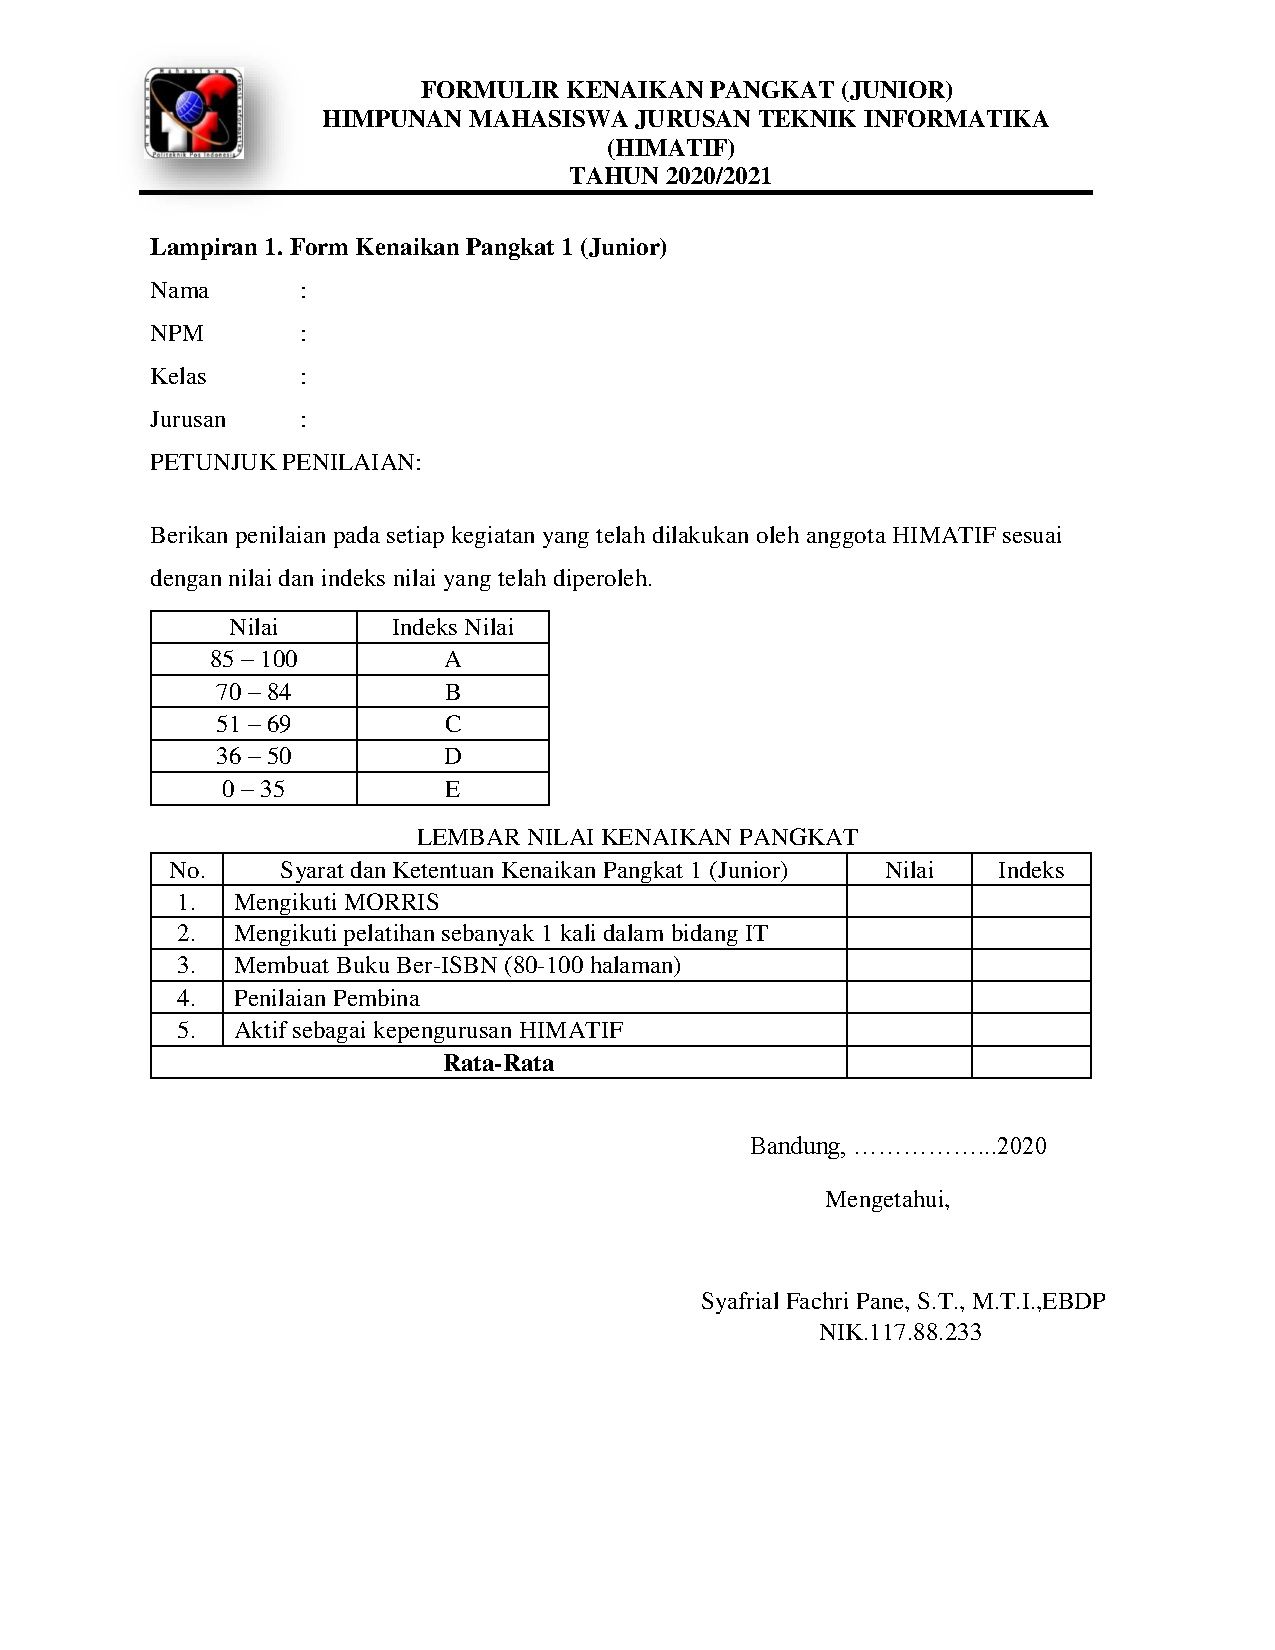
\includepdf[pages={1}]{pdf/PANGKAT1.pdf}      
\includepdf[pages={1}]{pdf/PANGKAt2.pdf} 
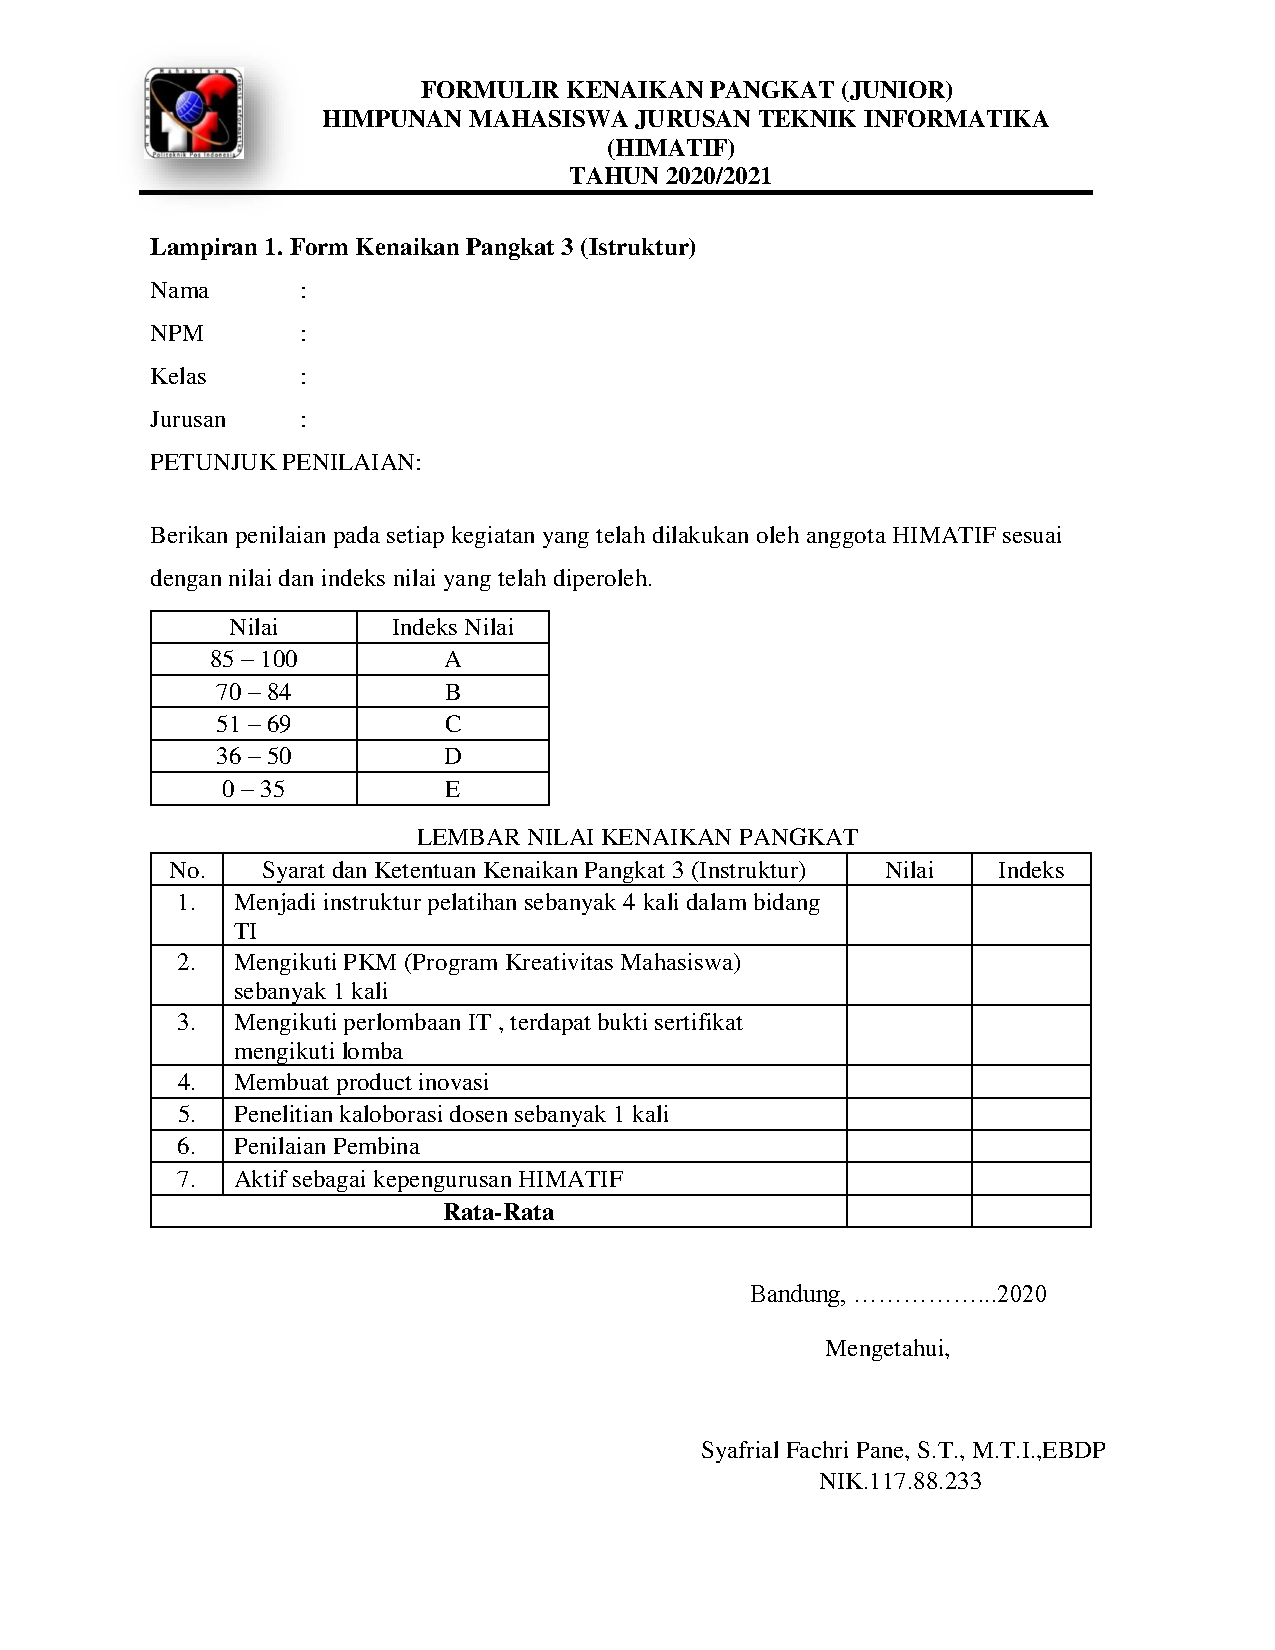
\includepdf[pages={1}]{pdf/PANGKAT3.pdf}
   
%next line adds the Bibliography to the contents page
\addcontentsline{toc}{chapter}{Bibliography}
%uncomment next line to change bibliography name to references
%\renewcommand{\bibname}{References}
%\bibliography{references}        %use a bibtex bibliography file refs.bib
\bibliographystyle{plain}  %use the plain bibliography style

\end{document}

